\documentclass[aspectratio=169,10pt]{beamer}

\usetheme{Madrid}
\setbeamertemplate{navigation symbols}{}
\setbeamertemplate{footline}[frame number]
\usepackage{hyperref}
\usepackage{amsmath}
\usepackage{amssymb}
\usepackage{array}
\usepackage{booktabs}
\usepackage{graphicx}
\usepackage{tabularx}
\usepackage{tikz}
\usetikzlibrary{arrows.meta,calc,positioning}

\graphicspath{{../../figures_ViT/}}

\definecolor{LectureBlue}{RGB}{13,76,100}
\definecolor{LectureTeal}{RGB}{0,118,122}
\definecolor{LectureGold}{RGB}{194,142,37}
\definecolor{Slate}{RGB}{58,68,84}
\definecolor{SoftGray}{RGB}{245,247,249}

\setbeamercolor{title}{fg=LectureBlue}
\setbeamercolor{subtitle}{fg=Slate}
\setbeamercolor{frametitle}{fg=LectureBlue,bg=LectureBlue!8}
\setbeamercolor{structure}{fg=LectureBlue}
\setbeamercolor{block title}{fg=white,bg=LectureBlue}
\setbeamercolor{block body}{fg=black,bg=SoftGray}
\setbeamercolor{alerted text}{fg=LectureGold}

\renewcommand{\arraystretch}{1.12}

\title{Vision Transformers (ViT) and Attention-Based Visual Architectures}
\subtitle{Data Science Graduate Course}
\author{}
\date{June 2026}

\begin{document}

% Slide 1: Title Slide
\begin{frame}[plain]
\begin{columns}[c,onlytextwidth]
\column{0.58\textwidth}
{\usebeamerfont{title}\color{LectureBlue}\inserttitle\par}
\vspace{0.4em}
{\usebeamerfont{subtitle}\color{Slate}\insertsubtitle\par}
\vspace{1.5em}
{\small \insertauthor \hfill \insertdate}

\column{0.38\textwidth}
\centering
\includegraphics[width=\linewidth]{vit.png}
\end{columns}
\end{frame}

% Slide 2: Table of Contents
\begin{frame}{Lecture Overview}
\begin{itemize}
    \item \textbf{Section 1: From CNNs to Visual Attention}
    \begin{itemize}
        \item Inherent limitations of local convolutions and translation equivariance
        \item The visual attention mechanism as a global paradigm shift
    \end{itemize}
    \item \textbf{Section 2: The Vision Transformer (ViT) Core Architecture}
    \begin{itemize}
        \item Image patching, linear projection, and the classification token
        \item Positional encodings, Multi-Head Self-Attention, and Pre-LN blocks
    \end{itemize}
    \item \textbf{Section 3: Inductive Biases and Training Dynamics}
    \begin{itemize}
        \item Spatial assumptions in CNNs vs. ViTs; sample efficiency and pretraining
    \end{itemize}
    \item \textbf{Section 4: Advanced Visual Transformer Architectures}
    \begin{itemize}
        \item Swin Transformer (shifted local windows and hierarchies)
        \item Deformable Attention Transformer (DAT) (content-adaptive sparse sampling)
    \end{itemize}
    \item \textbf{Section 5: Dense downstream Tasks \& Applications}
    \begin{itemize}
        \item Segmentation (TransUNet, Swin-Unet) and Object Detection (DETR)
    \end{itemize}
\end{itemize}
\end{frame}

% Slide 3: Section Divider - Section 1
\section{From CNNs to Transformers}
\begin{frame}
\centering
\vspace{0.25\textheight}
{\Huge Section 1: From CNNs to Transformers}
\end{frame}

% Slide 4: Limitations of Convolutional Architectures
\begin{frame}{Inherent Limitations of CNNs}
\begin{columns}[T,onlytextwidth]
\column{0.55\textwidth}
\begin{itemize}
    \item \textbf{Local Receptive Fields}: 
    \begin{itemize}
        \item Standard convolution layers only process pixels within a local neighborhood.
        \item Contextual relationships are established slowly through hierarchical stacking of pooling/downsampling.
    \end{itemize}
    \item \textbf{Locality Bias}:
    \begin{itemize}
        \item Assumes nearby features are strongly coupled while distant features are independent.
    \end{itemize}
    \item \textbf{Downstream Bottleneck}:
    \begin{itemize}
        \item Modeling global interactions and long-range dependencies is challenging in early layers.
    \end{itemize}
\end{itemize}

\column{0.40\textwidth}
\centering
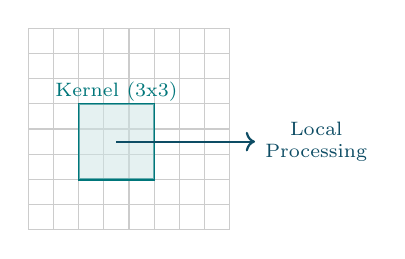
\begin{tikzpicture}[scale=0.8]
    % Draw an grid representing image pixels
    \draw[gray!40, step=0.4] (0,0) grid (3.2,3.2);
    % Local convolution kernel
    \draw[LectureTeal, thick] (0.8,0.8) rectangle (2.0,2.0);
    \node[LectureTeal, font=\scriptsize] at (1.4,2.2) {Kernel (3x3)};
    \fill[LectureTeal!20, opacity=0.5] (0.8,0.8) rectangle (2.0,2.0);
    % Draw receptive field arrows
    \draw[->, thick, LectureBlue] (1.4,1.4) -- (3.6,1.4) node[right, font=\scriptsize, align=center] {Local\\Processing};
\end{tikzpicture}
\end{columns}
\end{frame}

% Slide 5: The Visual Attention Paradigm Shift
\begin{frame}{The Visual Attention Paradigm Shift}
\begin{columns}[T,onlytextwidth]
\column{0.58\textwidth}
\begin{quote}
``The ability to dynamically highlight and use the salient parts of the information at hand... inspired by the human visual system.'' \\
--- Grace W. Lindsay, 2020
\end{quote}
\vspace{1.0em}
\begin{itemize}
    \item \textbf{Global Receptive Field}: 
    \begin{itemize}
        \item Self-attention allows each token (patch) to directly interact with all other tokens from the first layer.
        \item Spatial distance does not constrain learning.
    \end{itemize}
    \item \textbf{Content-Dependent Weighting}:
    \begin{itemize}
        \item Weights are dynamically computed based on the similarity between queries and keys, rather than fixed spatial filters.
    \end{itemize}
\end{itemize}

\column{0.38\textwidth}
\centering
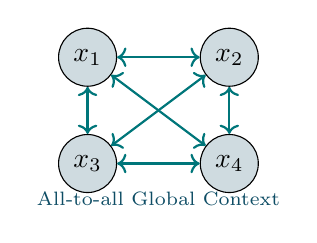
\begin{tikzpicture}[scale=0.9]
    % Draw nodes
    \node[draw, circle, fill=LectureBlue!20] (n1) at (0,1.5) {$x_1$};
    \node[draw, circle, fill=LectureBlue!20] (n2) at (2,1.5) {$x_2$};
    \node[draw, circle, fill=LectureBlue!20] (n3) at (0,0) {$x_3$};
    \node[draw, circle, fill=LectureBlue!20] (n4) at (2,0) {$x_4$};
    % Draw self-attention links
    \draw[<->, thick, LectureTeal] (n1) -- (n2);
    \draw[<->, thick, LectureTeal] (n1) -- (n3);
    \draw[<->, thick, LectureTeal] (n1) -- (n4);
    \draw[<->, thick, LectureTeal] (n2) -- (n3);
    \draw[<->, thick, LectureTeal] (n2) -- (n4);
    \draw[<->, thick, LectureTeal] (n3) -- (n4);
    \node[font=\scriptsize, text=LectureBlue] at (1,-0.5) {All-to-all Global Context};
\end{tikzpicture}
\end{columns}
\end{frame}

% Slide 6: Section Divider - Section 2
\section{The Vision Transformer (ViT) Core Architecture}
\begin{frame}
\centering
\vspace{0.25\textheight}
{\Huge Section 2: The Vision Transformer (ViT) Core Architecture}
\end{frame}

% Slide 7: Image Patching & Linear Projection
\begin{frame}{Image Patching and Linear Projection}
\begin{columns}[T,onlytextwidth]
\column{0.55\textwidth}
The Vision Transformer (Dosovitskiy et al., 2021) models images as sequences of patches:
\begin{itemize}
    \item \textbf{Patching Operator}:
    Splits image $\mathbf{x} \in \mathbb{R}^{H \times W \times C}$ into $N = HW/P^2$ patches $\mathbf{x}_p^i \in \mathbb{R}^{P^2 C}$ (e.g., $P=4 \implies N = 64$ patches for $32\times32$ image).
    \item \textbf{Linear Projection}:
    Projects each flattened patch to dimension $D$:
    \[
    \mathbf{z}_p^i = \mathbf{x}_p^i \mathbf{E}, \quad \mathbf{E} \in \mathbb{R}^{(P^2 C) \times D}
    \]
    \item \textbf{Complexity Avoidance}:
    Self-attention over raw pixels $\mathcal{O}((HW)^2)$ is intractable. Patching reduces token count to $N$, ensuring computational feasibility.
\end{itemize}

\column{0.40\textwidth}
\centering
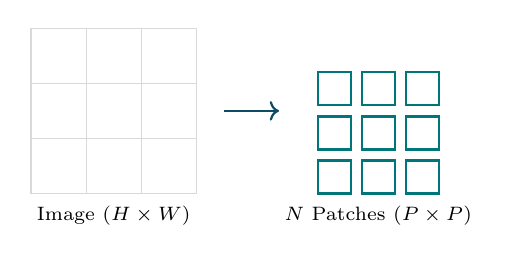
\begin{tikzpicture}[scale=0.7]
    % Draw original grid
    \draw[gray!30] (0,0) grid (3,3);
    \node[font=\scriptsize] at (1.5, -0.4) {Image ($H \times W$)};
    % Arrow
    \draw[->, thick, LectureBlue] (3.5, 1.5) -- (4.5, 1.5);
    % Patches
    \begin{scope}[xshift=5.2cm]
        \foreach \x in {0, 0.8, 1.6} {
            \foreach \y in {0, 0.8, 1.6} {
                \draw[LectureTeal, thick] (\x, \y) rectangle (\x+0.6, \y+0.6);
            }
        }
        \node[font=\scriptsize] at (1.1, -0.4) {$N$ Patches ($P \times P$)};
    \end{scope}
\end{tikzpicture}
\end{columns}
\end{frame}

% Slide 8: Classification Token & Positional Encodings
\begin{frame}{Classification Token and Positional Encodings}
\begin{columns}[T,onlytextwidth]
\column{0.55\textwidth}
\begin{itemize}
    \item \textbf{Classification token (\texttt{[CLS]})}:
    \begin{itemize}
        \item A learnable embedding $\mathbf{x}_{\text{class}} \in \mathbb{R}^D$ is prepended to the patch embeddings.
        \item Serving as the query to gather classification information across all other patch embeddings.
        \item The final state of the \texttt{[CLS]} token at the encoder output ($\mathbf{z}_L^0$) is mapped to the output classification head.
    \end{itemize}
    \item \textbf{Positional Encodings}:
    \begin{itemize}
        \item Self-attention does not preserve sequence order.
        \item We add learnable, 1D positional parameters $\mathbf{E}_{\text{pos}} \in \mathbb{R}^{(N+1)\times D}$ to incorporate spatial structure.
        \[
        \mathbf{z}_0 = [\mathbf{x}_{\text{class}}; \mathbf{x}_p^1 \mathbf{E}; \dots; \mathbf{x}_p^N \mathbf{E}] + \mathbf{E}_{\text{pos}}
        \]
    \end{itemize}
\end{itemize}

\column{0.40\textwidth}
\centering
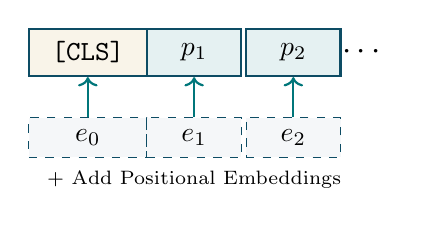
\begin{tikzpicture}[scale=0.9]
    \node[draw=LectureBlue, thick, fill=LectureGold!10, minimum width=1.5cm, minimum height=0.6cm] (cls) at (0,1.2) {\texttt{[CLS]}};
    \node[draw=LectureBlue, thick, fill=LectureTeal!10, minimum width=1.2cm, minimum height=0.6cm] (p1) at (1.5,1.2) {$p_1$};
    \node[draw=LectureBlue, thick, fill=LectureTeal!10, minimum width=1.2cm, minimum height=0.6cm] (p2) at (2.9,1.2) {$p_2$};
    \node[font=\large] at (3.9, 1.2) {$\cdots$};
    
    \node[draw=LectureBlue, dashed, minimum width=1.5cm, minimum height=0.5cm, fill=SoftGray] (pos_cls) at (0,0) {$e_0$};
    \node[draw=LectureBlue, dashed, minimum width=1.2cm, minimum height=0.5cm, fill=SoftGray] (pos_p1) at (1.5,0) {$e_1$};
    \node[draw=LectureBlue, dashed, minimum width=1.2cm, minimum height=0.5cm, fill=SoftGray] (pos_p2) at (2.9,0) {$e_2$};
    
    \draw[->, thick, LectureTeal] (pos_cls) -- (cls);
    \draw[->, thick, LectureTeal] (pos_p1) -- (p1);
    \draw[->, thick, LectureTeal] (pos_p2) -- (p2);
    
    \node[font=\scriptsize] at (1.5,-0.6) {+ Add Positional Embeddings};
\end{tikzpicture}
\end{columns}
\end{frame}

% Slide 9: Self-Attention Mechanism (Mathematical Details)
\begin{frame}{Self-Attention Mechanism: Mathematical Details}
\begin{itemize}
    \item Projection of the input matrix $X \in \mathbb{R}^{(N+1)\times D}$ using query, key, and value weight matrices:
    \[
    Q = X\mathbf{W}_Q, \quad K = X\mathbf{W}_K, \quad V = X\mathbf{W}_V, \quad \mathbf{W}_Q, \mathbf{W}_K, \mathbf{W}_V \in \mathbb{R}^{D \times D_k}
    \]
    \item Computing attention weights using Query-Key scaled dot-products:
    \[
    A = \text{softmax}\left(\frac{QK^T}{\sqrt{d_k}}\right), \quad A \in \mathbb{R}^{(N+1)\times (N+1)}
    \]
    \item The output is a weighted sum of representation values:
    \[
    \text{Attention}(Q, K, V) = A V
    \]
\end{itemize}
\begin{block}{Why Scale by $\sqrt{d_k}$?}
Without scaling, for large projection dimensions $d_k$, the dot product values grow large in magnitude. This pushes the softmax function into regions with extremely small gradients (vanishing gradient problem). Dividing by $\sqrt{d_k}$ maintains stable variance.
\end{block}
\end{frame}

% Slide 10: Multi-Head Self-Attention (MHSA)
\begin{frame}{Multi-Head Self-Attention (MHSA)}
\begin{columns}[T,onlytextwidth]
\column{0.52\textwidth}
\begin{itemize}
    \item Allows the model to attend to different representation subspaces at different positions.
    \[
    \text{MHSA}(Q, K, V) = [\mathbf{h}_1; \dots; \mathbf{h}_h]\mathbf{W}^O
    \]
    where $\mathbf{h}_i = \text{Attention}(Q\mathbf{W}_i^Q, K\mathbf{W}_i^K, V\mathbf{W}_i^V)$
    \item $\mathbf{W}_i^Q, \mathbf{W}_i^K \in \mathbb{R}^{D \times D_k}$, $\mathbf{W}_i^V \in \mathbb{R}^{D \times D_v}$, and $\mathbf{W}^O \in \mathbb{R}^{hD_v \times D}$.
    \item Multi-head scaling balances representation capacity and prevents query-key collapse.
\end{itemize}

\column{0.44\textwidth}
\centering
\includegraphics[width=\linewidth]{vit_ex.png}
\end{columns}
\end{frame}

% Slide 11: Transformer Encoder Block: Pre-LN Architecture
\begin{frame}{Pre-LN vs. Post-LN Block Layout}
\begin{columns}[T,onlytextwidth]
\column{0.55\textwidth}
ViT adopts the \textbf{Pre-Layer Normalization} (Pre-LN) block structure (Xiong et al., 2020).
\begin{itemize}
    \item \textbf{Post-LN (Standard Transformer)}:
    \newline {\small $\mathbf{x}'_l = \text{LN}(\mathbf{x}_{l-1} + \text{MHSA}(\mathbf{x}_{l-1}))$, \quad $\mathbf{x}_l = \text{LN}(\mathbf{x}'_l + \text{MLP}(\mathbf{x}'_l))$}
    \item \textbf{Pre-LN (ViT Block)}:
    \newline {\small $\mathbf{x}'_l = \mathbf{x}_{l-1} + \text{MHSA}(\text{LN}(\mathbf{x}_{l-1}))$, \quad $\mathbf{x}_l = \mathbf{x}'_l + \text{MLP}(\text{LN}(\mathbf{x}'_l))$}
    \item \textbf{Advantage of Pre-LN}:
    \begin{itemize}
        \item Normalization on the residual branch prior to layer execution prevents vanishing/exploding gradients.
        \item Removes the necessity of a learning rate warm-up stage.
    \end{itemize}
\end{itemize}

\column{0.42\textwidth}
\centering
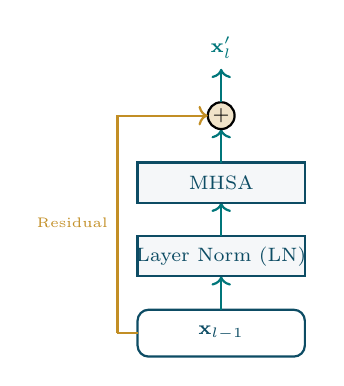
\begin{tikzpicture}[scale=0.85, font=\scriptsize]
    % Pre-LN Flowchart
    \draw[thick, LectureBlue, rounded corners] (0,0) rectangle (2.5,0.7) node[midway] {$\mathbf{x}_{l-1}$};
    \draw[->, thick, LectureTeal] (1.25,0.7) -- (1.25,1.2);
    \draw[thick, LectureBlue, fill=SoftGray] (0,1.2) rectangle (2.5,1.8) node[midway] {Layer Norm (LN)};
    \draw[->, thick, LectureTeal] (1.25,1.8) -- (1.25,2.3);
    \draw[thick, LectureBlue, fill=SoftGray] (0,2.3) rectangle (2.5,2.9) node[midway] {MHSA};
    \draw[->, thick, LectureTeal] (1.25,2.9) -- (1.25,3.4);
    
    % Sum node
    \draw[thick, fill=LectureGold!25] (1.25,3.6) circle (0.2) node {$+$};
    \draw[->, thick, LectureTeal] (1.25,3.8) -- (1.25,4.3) node[above] {$\mathbf{x}'_l$};
    
    % Residual line
    \draw[thick, LectureGold, ->] (-0.3, 0.35) -- (-0.3, 3.6) -- (1.05,3.6);
    \draw[thick, LectureGold] (0, 0.35) -- (-0.3, 0.35);
    \node[font=\tiny, left, LectureGold] at (-0.3, 2.0) {Residual};
\end{tikzpicture}
\end{columns}
\end{frame}

% Slide 12: Section Divider - Section 3
\section{Inductive Biases and Training Dynamics}
\begin{frame}
\centering
\vspace{0.25\textheight}
{\Huge Section 3: Inductive Biases and Training Dynamics}
\end{frame}

% Slide 13: Inductive Biases: CNNs vs. ViTs
\begin{frame}{Inductive Biases: Convolutions vs. Self-Attention}
\begin{itemize}
    \item \textbf{Inductive Bias}: The set of assumptions a learning algorithm uses to predict outputs for unseen inputs.
\end{itemize}
\vspace{0.5em}
\begin{tabularx}{\textwidth}{>{\bfseries\color{LectureBlue}}p{0.22\textwidth} X X}
\toprule
Property & Convolutional Networks (CNNs) & Vision Transformers (ViTs) \\
\midrule
Locality & Nearby pixels are highly correlated. Spatial relationships are hard-coded. & Weak local bias. Global receptive field from layer 0. Spatial relations must be learned. \\
Translation Invariance & Filter weights are shared spatially. Shifted inputs yield shifted feature maps. & Permutation equivariant. Relies purely on positional encoding parameters to learn geometry. \\
Data Requirement & Generalizes well on small datasets. & Requires massive datasets or strong pretraining to generalize. \\
\bottomrule
\end{tabularx}
\end{frame}

% Slide 14: Data Efficiency & The Role of Pretraining
\begin{frame}{Data Efficiency and The Role of Pretraining}
\begin{columns}[T,onlytextwidth]
\column{0.52\textwidth}
\begin{itemize}
    \item \textbf{Small Dataset Gap (CIFAR-10)}:
    \begin{itemize}
        \item CNNs (e.g. ResNets) easily reach $\sim 90\%$ validation accuracy from scratch.
        \item Vision Transformers (ViT) underperform, reaching only $\sim 75\%$ from scratch.
    \end{itemize}
    \item \textbf{Why?}:
    \begin{itemize}
        \item CNNs have a strong translation equivariance and locality bias.
        \item ViT must learn spatial grid structures solely from sparse classification signals.
    \end{itemize}
    \item \textbf{Scale Transition}:
    \begin{itemize}
        \item At massive scale (ImageNet, JFT-300M), ViT outperforms CNNs, showing higher capacity.
    \end{itemize}
\end{itemize}

\column{0.44\textwidth}
\centering
\includegraphics[width=0.9\linewidth]{vit_cnn.png}
\end{columns}
\end{frame}

% Slide 15: Section Divider - Section 4
\section{Advanced Visual Transformer Architectures}
\begin{frame}
\centering
\vspace{0.25\textheight}
{\Huge Section 4: Advanced Visual Transformer Architectures}
\end{frame}

% Slide 16: Swin Transformer: Shifted Windows
\begin{frame}{Swin Transformer: Shifted Windows}
\begin{columns}[T,onlytextwidth]
\column{0.55\textwidth}
The Swin (Shifted Window) Transformer (Liu et al., 2021) addresses the $\mathcal{O}(N^2)$ quadratic complexity limitation of global attention.
\begin{itemize}
    \item \textbf{Window-based Attention}:
    \begin{itemize}
        \item Images are partitioned into non-overlapping local windows (e.g. $7 \times 7$ patches).
        \item Self-attention is computed *only* within each local window.
        \item Complexity drops from $\mathcal{O}(N^2)$ to $\mathcal{O}(M^2 N)$ (linear in image size).
    \end{itemize}
    \item \textbf{Shifted Window Partitioning}:
    \begin{itemize}
        \item Alternating layers shift the window partition boundary by $(\lfloor M/2 \rfloor, \lfloor M/2 \rfloor)$.
        \item This introduces connections between adjacent local windows from previous layers, enabling cross-window context.
    \end{itemize}
\end{itemize}

\column{0.40\textwidth}
\centering
\includegraphics[width=\linewidth]{swin_compare.png}
\end{columns}
\end{frame}

% Slide 17: Swin Transformer: Hierarchical Feature Maps
\begin{frame}{Swin Transformer: Hierarchical Feature Maps}
\begin{columns}[T,onlytextwidth]
\column{0.52\textwidth}
\begin{itemize}
    \item Unlike ViT which maintains a constant sequence length, Swin builds a hierarchical representation.
    \item \textbf{Patch Merging}:
    \begin{itemize}
        \item Concatenates neighboring patches (e.g., $2 \times 2$ groupings).
        \item Reduces spatial resolution by half ($H/2 \times W/2$) and doubles representation dimensionality.
    \end{itemize}
    \item \textbf{Pyramid Hierarchy}:
    \begin{itemize}
        \item Mimics CNN hierarchies (e.g. ResNet feature pyramid).
        \item Essential for dense downstream vision tasks (object detection, segmentation) requiring multi-scale feature maps.
    \end{itemize}
\end{itemize}

\column{0.44\textwidth}
\centering
\includegraphics[width=\linewidth]{swin_arch.png}
\end{columns}
\end{frame}

% Slide 18: Deformable Attention Transformer (DAT)
\begin{frame}{Deformable Attention Transformer (DAT)}
\begin{columns}[T,onlytextwidth]
\column{0.52\textwidth}
\begin{itemize}
    \item Global attention is computationally redundant; local window attention is spatially rigid.
    \item \textbf{Deformable Attention} (Xia et al., 2022):
    \begin{itemize}
        \item Dynamically shifts the attention region based on content, sampling only a sparse set of keys/values.
    \end{itemize}
    \item \textbf{Mechanism}:
    \begin{itemize}
        \item Defines a uniform grid of reference points.
        \item Offset prediction network outputs displacements $\Delta p$ for each reference point based on queries.
        \item Keys and values are bilinearly sampled from offset coordinates.
    \end{itemize}
    \item Typically adopted only in deeper stages of the backbone to save compute.
\end{itemize}

\column{0.44\textwidth}
\centering
\includegraphics[width=\linewidth]{dat_arch.png}
\end{columns}
\end{frame}

% Slide 19: Section Divider - Section 5
\section{Downstream Vision Applications}
\begin{frame}
\centering
\vspace{0.25\textheight}
{\Huge Section 5: Downstream Vision Applications}
\end{frame}

% Slide 20: Medical Image Segmentation (TransUNet \& Swin-Unet)
\begin{frame}{Medical Image Segmentation: TransUNet and Swin-Unet}
\begin{columns}[T,onlytextwidth]
\column{0.52\textwidth}
Transformers excel in capturing global context, which is highly valuable in medical imaging (CT/MRI segmentation).
\begin{itemize}
    \item \textbf{TransUNet} (Chen et al., 2021):
    \begin{itemize}
        \item A hybrid architecture. CNN extracts high-resolution spatial feature maps.
        \item Transformer bottleneck encodes global self-attention context.
        \item CNN decoder restores resolution via skip connections.
    \end{itemize}
    \item \textbf{Swin-Unet} (Cao et al., 2021):
    \begin{itemize}
        \item A pure Transformer U-Net.
        \item Employs hierarchical Swin Transformer blocks for both encoding and decoding (patch expanding).
    \end{itemize}
\end{itemize}

\column{0.44\textwidth}
\centering
\includegraphics[height=0.34\textheight,keepaspectratio]{transunet.png}
\vspace{0.3em}
\includegraphics[height=0.34\textheight,keepaspectratio]{swinunet.png}
\end{columns}
\end{frame}

% Slide 21: Object Detection (DETR \& Deformable DETR)
\begin{frame}{Object Detection: DETR and Deformable DETR}
\begin{columns}[T,onlytextwidth]
\column{0.52\textwidth}
\begin{itemize}
    \item \textbf{DETR} (Carion et al., 2020):
    \begin{itemize}
        \item Replaces hand-crafted anchors, proposals, and Non-Maximum Suppression (NMS) with an end-to-end set prediction task.
        \item A CNN backbone extracts image features, processed by a Transformer Encoder-Decoder.
        \item Decodes a fixed set of $M$ bounding boxes using learnable \textbf{object queries}.
    \end{itemize}
    \item \textbf{Deformable DETR} (Zhu et al., 2021):
    \begin{itemize}
        \item Combines multi-scale spatial pyramid features and sparse deformable attention.
        \item Speeds up DETR convergence by up to 10x and handles high-resolution features efficiently.
    \end{itemize}
\end{itemize}

\column{0.44\textwidth}
\centering
\includegraphics[width=\linewidth]{ob_DETR.png}
\vspace{0.4em}
\includegraphics[width=\linewidth]{ob_deform_DETR.png}
\end{columns}
\end{frame}

% Slide 22: Conclusion & Summary
\begin{frame}{Conclusion and Summary}
\begin{itemize}
    \item \textbf{Convolutions to Self-Attention}:
    \begin{itemize}
        \item Self-attention allows dynamic global context extraction, contrasting with CNN's local filter boundaries.
    \end{itemize}
    \item \textbf{Inductive Bias vs. Representation Capacity}:
    \begin{itemize}
        \item CNNs possess translation equivariance and locality, making them sample-efficient on small datasets.
        \item ViTs have fewer spatial assumptions, providing superior capacity when trained on large-scale datasets.
    \end{itemize}
    \item \textbf{Hybrid \& Hierarchical Advancements}:
    \begin{itemize}
        \item Architectures like Swin Transformer and Deformable Attention (DAT) combine spatial hierarchies and linear attention constraints to excel in dense, high-resolution downstream tasks.
    \end{itemize}
\end{itemize}
\end{frame}

% Slide 23: References
\begin{frame}{Key References}
\footnotesize
\begin{itemize}
    \item \textbf{Vision Transformer (ViT)}: \\
    Dosovitskiy, A., et al. ``An image is worth 16x16 words: Transformers for image recognition at scale.'' \textit{ICLR}, 2021.
    \item \textbf{Swin Transformer}: \\
    Liu, Z., et al. ``Swin transformer: Hierarchical vision transformer using shifted windows.'' \textit{ICCV}, 2021.
    \item \textbf{Deformable Attention Transformer (DAT)}: \\
    Xia, Z., et al. ``Vision transformer with deformable attention.'' \textit{CVPR}, 2022.
    \item \textbf{Pre-Layer Normalization}: \\
    Xiong, R., et al. ``On layer normalization in the transformer architecture.'' \textit{ICML}, 2020.
    \item \textbf{Detection Transformer (DETR)}: \\
    Carion, N., et al. ``End-to-end object detection with transformers.'' \textit{ECCV}, 2020.
    \item \textbf{TransUNet}: \\
    Chen, J., et al. ``Transunet: Transformers make strong encoders for medical image segmentation.'' \textit{arXiv:2102.04306}, 2021.
\end{itemize}
\end{frame}

\end{document}
